%%%%%%%%%%%%%%%%%%%%%%%%%%%%%%%%%%%%%%%%%%%%%%%%%%%%%%%%%%%%%%%%%%
%%%%%%%% ICML 2013 EXAMPLE LATEX SUBMISSION FILE %%%%%%%%%%%%%%%%%
%%%%%%%%%%%%%%%%%%%%%%%%%%%%%%%%%%%%%%%%%%%%%%%%%%%%%%%%%%%%%%%%%%
\documentclass{article}

% For figures
\usepackage{graphicx} % more modern
\usepackage{subfigure}
\usepackage{natbib}
\usepackage{algorithm}
\usepackage{algorithmic}
\usepackage{hyperref}
\usepackage{tikz}
\usepackage{amsmath}
\newcommand{\theHalgorithm}{\arabic{algorithm}}
\usepackage{icml2013}

\icmltitlerunning{Modeling Patient Disease Dynamics}
\usetikzlibrary{shapes,arrows,automata}

\begin{document}

\twocolumn[
\icmltitle{Semiparametric Clustering Methods for\\ Modeling Chronic Disease Dynamics}

\icmlauthor{Suzanne Tamang}{suzanne.tamang@gmail.com}
\icmladdress{Graduate Center City University of New York,
            314159 Pi St., Palo Alto, CA 94306 USA}
\icmlauthor{Your CoAuthor's Name}{email@coauthordomain.edu}
\icmladdress{Their Fantastic Institute,
            27182 Exp St., Toronto, ON M6H 2T1 CANADA}
\icmlkeywords{temporal clustering, clinical data, continuous time dynamic Bayesian networks, nonparametric Bayesian methods}

\vskip 0.3in
]

\begin{abstract}
The availability of clinical data repositories presents new opportunities for improving health care quality and reducing costs.  However, the secondary function of these data sources as research tools presents challenges for longitudinal data analysis.  Rather than use the sequences directly, we extend the semiparametric clustering framework to build probabilistic models, abstractions, of these sequences using continuous-time Markov models.  This provides a principled way of transforming arbitrarily sampled, irregular length clinical observations to serve as input for a nonparametric Bayesian clustering method. Our results indicate over a 20\% relative improvement on a benchmark and recognizable differences that can be visualized.
\end{abstract}

\section{Motivation}
\label{intro}
The most significant issues facing the US health care system in the coming years includes: major aging, the massive growth of chronic diseases, and not enough caregivers.  Increasing health care costs and quality issues already pose substantial issues and unless sustainable solutions can be developed our the US healthcare system will become increasingly stressed.

One proposition for transforming healthcare is to make it `data-driven' and has resulted in numerous government and private initiatives aiming to make meaningful use of digital health data.  Advocates hope that the richness of available patient data contained in these collections will enable a feedback loop of new knowledge discovery and translation to practice, supporting the engineering of a better and better health care system. There is an urgent need to demonstrate the cost-benefit of maintaining petabytes of patient data, and an important role for probabilistic learning algorithms that can assist in the discovery new knowledge from these noisy, heterogenous, fragmented data collections.

Here we provide one way to approach
data-driven care.  To model chronic disease dynamics, which may evolve slowly, over years, we extend the semiparametric clustering framework of Jebara et al.~\cite{JebSonTha07a} for learning patient and population level disease characteristics from arbitrarily sampled longitudinal patient data.  Specifically, we use parametric models based on continuous time Markov models paired with nonparmetric Bayesian clustering and we show results for two distinct data sets.

We describe the background for our work in Section~\ref{prelims}.  Our contribution and methods are detailed in Section~\ref{sp}.  The rest of the paper describes: two applications in Section~\ref{expts}, experimental results in Section~\ref{clin}, and conclusions for our work in Section~\ref{conc}.


\section{Preliminaries}
\label{prelims}
Clustering is a pervasive and natural human activity that is used for a variety of tasks. Typically, we use it to group similar objects together so that we can assign characteristics that are useful for their definition.  %It's important to note that agreement among experts on the `correct' assignment of items can produce controversy.  For example, there have been extreme departures in the biological sciences attributed to defining the membership of some organisms that cannot be definitively resolved.
Computational clustering algorithms aim to divide data into groups that are meaningful or useful, and improving existing techniques has been the focus of considerable research in machine learning.  At the minimal level, automated clustering can be viewed as a preprocessing method, or as an exploratory analysis technique that informs more targeted hypotheses.

\subsection{Semiparametric Time Series Clustering}
Temporal information provides critical context for diagnosis, prognosis and disease management, especially in the case of chronic conditions that can evolve at different rates among patients, and persist for years.   Although clinically significant work applying exploratory techniques for patient and population level disease modeling has been demonstrated~\cite{Saria09,Marlin12}, it is most appropriate for methods based on physiological signals collected in the critical care setting.  Chronic disease progression can take months or years to manifest, and longer-term trends instead of significant features can have increased importance.  Also, in the low frequency sampling setting, the sampling scheme may be unknown, data is more sparse, and collected over longer durations.

In the \emph{semi-parametric clustering framework}, a parametric model of the underlying dynamic process provides useful assumptions for abstracting temporal measurement, and is paired with a nonparametric method used to cluster the abstractions.  Figure~\ref{semipar} provides an overview of this approach.

\begin{figure}[t]
\vskip 0.2in
\begin{center}
\centerline{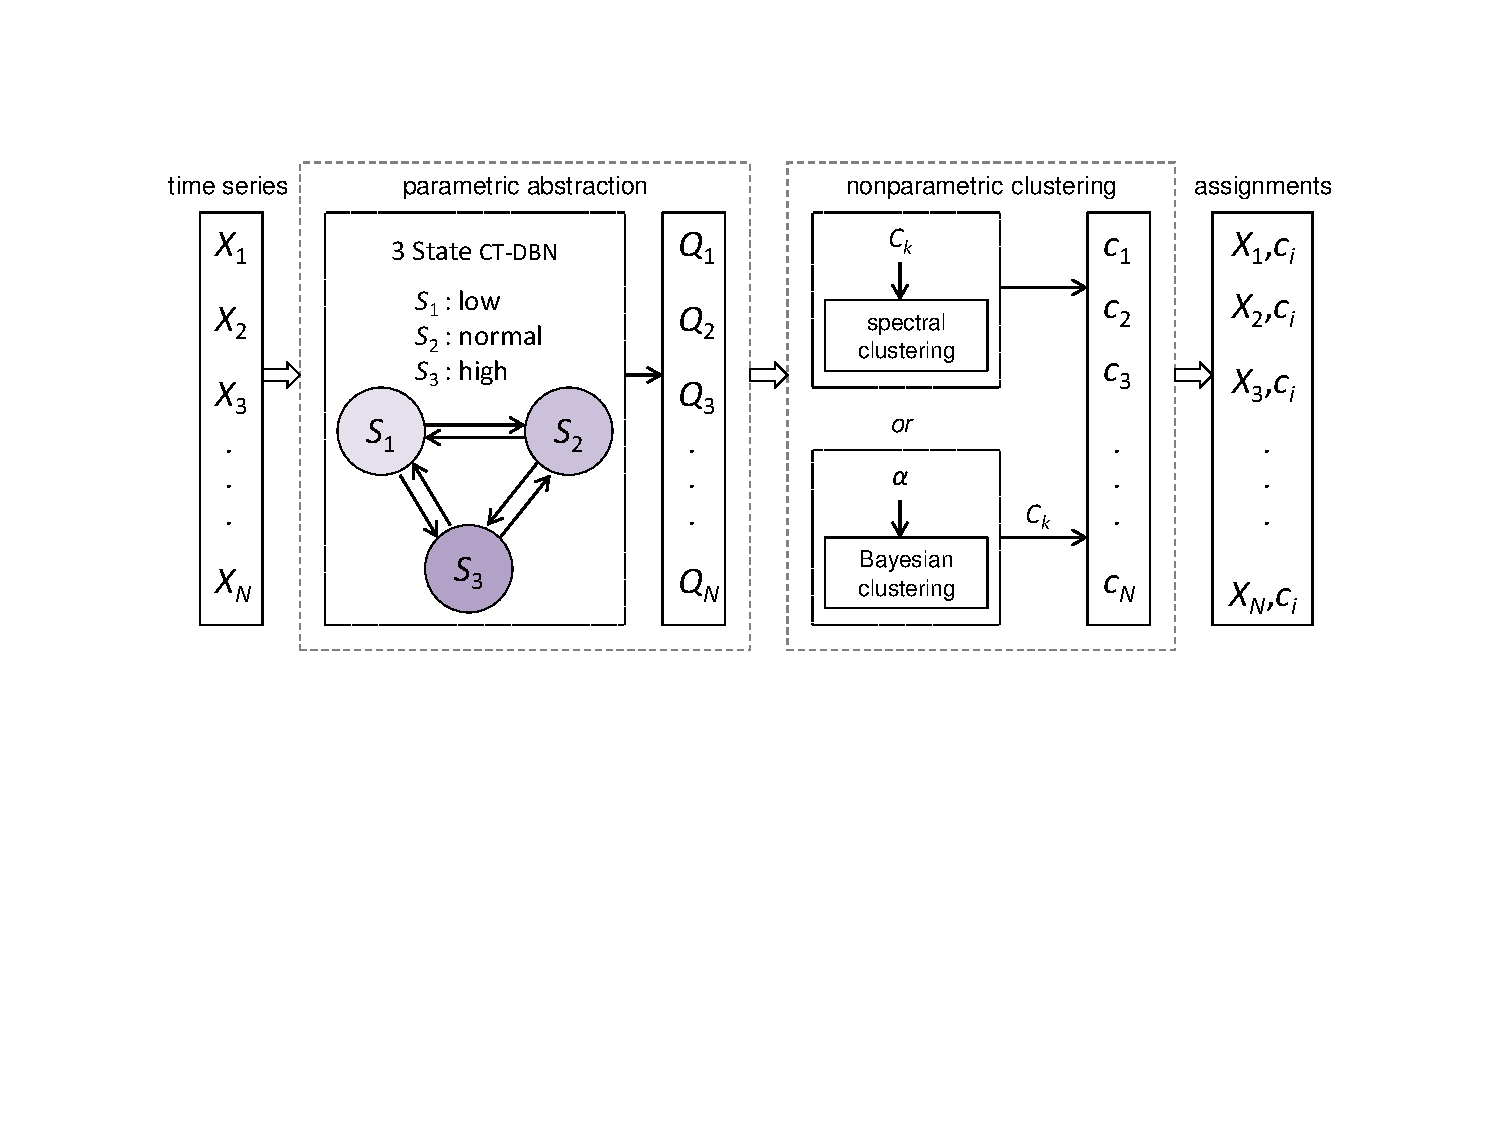
\includegraphics[width=\columnwidth]{fig/semipoverview.jpg}}
\caption{Semiparametric Clustering}
\label{semipar}
\end{center}
\vskip -0.2in
\end{figure}

%temporal clustering
The first step entails temporal abstraction using a parametric model to transform a set of raw time series, $X_1,X_2,...,X_N$, into a more manageable form for traditional multivariate clustering algorithms. It entails learning each patients model-specific parameters, $Q_1,Q_2,...,Q_N$, from the time series observations.  The second step is nonparametric clustering.  Spectral methods are typically used in the semiparametric framework, which requires determining the number of clusters, $k$, in advance.  In this work, we extend the clustering component to the nonparametric Bayesian setting, allowing for the number of clusters to be expressed as a function of the sample size.


\subsection{Continuous and Discrete-time Models}
 By default Markov models and dynamic Bayesian networks (DBNs), of which a hidden Markov model (HMM) is the simplest representation, discretize the time trajectory into uniform length contiguous segments, that are assumed to be approximately Markovian to enable tractable inference.  The smallest temporal granularity among all sequences, $\Delta$, denotes a fixed length interval that is repeated at each time slice, where a the template models is also repeated.

 Although discrete-time models are suitable in many cases, there are two key limitations that have been noted in graphical modeling problems~\cite{Nodelman02} and we describe their relevance to modeling EHR data. First, if the underlying health phenomena progresses in individuals at different rates, one granularity must be used to express time steps for the entire system. Second, when data is unavailable, intervening time slices must still be represented.  When data is sparse, this forces the assumption of many unknown values that are propagated through the discrete time model's transition matrix at each $\Delta t$ without support.

%Various examination schemes are possible in the clinical setting and their impact on longitudinal chronic disease studies have been studied\cite{gruger}.  Fixed, random and examination schemes for severely ill patients under a doctor's care have been shown to be non-informative.  However, \emph{self-selection}, which is often driven by a patient's need to see formal care when they are in a poor condition is informative, indicating the missing at random assumption for longitudinal analysis of chronic disease patients is not realistic.  An EHR that provides a comprehensive view of a patients clinical care, makes it more likely to assume that missing data corresponds with a patient absent of disease related symptoms.  However, the fragmentation of patient data mirrors that of the larger US health care system.  A patient seeking care at another provider is not easily known, and estimating values in the absence can be problematic.  A recent simulation study that modeled patient data with DT-HMMs~\cite{YehCS12} assessed the impact of missing observations for various scenarios, and concluded that there is substantial impact on parameter estimates when the data is not missing completely at random and the missing data mechanism in non-ignorable.

When there are no natural time slices, continuous-time DBNs (CT-DBNs)~\cite{Nodelman02} can be used to more directly reflect sequential dependencies, and avoid discretizing the time intervals.  Notably, the class of probabilistic graphical models known in epidemiology and biostatistics as Multi-state models (MSMs), some of which qualify as CT-DBNs, were developed independently of work in computer science and share their foundation in stochastic process theory.

%For chronic disease modeling, biostaticians have noted that discrete time model are an inappropriate citing arbitrary sampling that must be considered and the time course of progression, which may not be linear and evolves at different rates among patients. CT-DBNs, primarily continuous-time hidden Markov models (HMM) have be used to model health decline for variety of conditions including lung disease, and HIV~\cite{Jackson10}.  Also, CT-HMMs have been applied to discovering disease relationships and to overcome the drawbacks of discrete-time models for predicting disease interactions in mental health, and their effectiveness has been demonstrated on a recent, large-scale study~\cite{Murillo}.

%Notably, the class of probabilistic graphical models known in epidemiology and biostatistics as Multi-state models (MSMs).  Not all MSM models are CT-DBNs.  However, many of their extensions for modeling latent variables and covariances, which can be viewed as specialized instance of CT-DBNs applied for modeling disease dynamics.  Although they were developed independently of work in computer science, they share the same grounding in stochastic process theory and share similarities for representation, learning and inference.  MSM were motivated by the limitations of discrete time stochastic processes for modeling disease dynamics from longitudional data with missing observations, or \emph{panel data}~\cite{Jackson10}.

MSMs have a set of rules that govern their design and interpretation and have be used to model a variety of diseases including cardiac disease, cancer, and HIV~\cite{Jackson10}. In terms of structure, nodes represent disease states that are ordered progressively to reflect stages in a disease trajectory.  A patient with chronic diseases may traverse these nodes as their disease progresses, and typical MSM states correspond with `healthy', `diseased', and `diseased with complications'.  In the case of applications to survival analysis, a final absorbing state that has no outbound transitions is used to indicate death. Also, for modeling latent states, is common for an MSM emission matrix to reflect diagnostic misclassification error, and there are techniques to estimate initial values based on sensitivity and specificity.



%\section{Related Work}
%\label{rel}
%
%semi-parametric framework
Generative probabilistic frameworks for abstracting time series for standard multi-variate techniques have been broadly described~\cite{Cadez00ageneral}, and are motivated by the limitations of distance functions to approximate the variable amounts of temporal available for comparing observations in complex problems.  Semi-parametric clustering can be viewed as a specification in this broad category that uses DBNs, commonly hidden Markov models and their variants, to embed parametric assumptions about time and the relationships among variables to represent the underlying dynamical systems being studied.  Most applications pair abstractions with spectral clustering, and recent applications to motion capture data~\cite{JebSonTha07a} show performance comparable to that of supervised learning.

%timeseries using PGMs for abstraction
 Recent work applying probabilistic machine learning applications for the temporal modeling of high and medium frequency physiological signals collected in the critical care environment have demonstrated prognostic relevance.  Recent work used a nonparametric Bayesian framework to discover dynamical features from time series using a Bayesian non-parametric framework to capture higher-level concepts related to infant mortality, discovering dynamical features from time series~\cite{Saria09}. Also for unsupervised pattern discovery, other work used probabilistic clustering models to address uncertain and sparse sampled time series data~\cite{Marlin12}.  However, chronic disease progression can take weeks, months or years to manifest and these methods do not address the low frequency setting where trends instead of significant features can have increased importance, and observations are recorded over much longer durations.

\section{Semiparametric Clustering Method}
\label{sp}
Regardless of the temporal mining task, the first step of an algorithm is to transform,
or abstract, the raw data into a more concise representation, preserving as much of the
information contained in the original sequence as possible.

\subsection{Continuous Time (CT) Model Abstraction}
As mentioned above, Markov models and DBNs require that continuous time is represented as a series of uniform length units equal to the smallest time granularity in any observed sequence. When data is missing or otherwise incomplete, information is still propagated throughout the model for every time step. It has been shown that when data is not missing at random, which often the case in clinical data, it can result in significantly more EM steps to learn the model parameters, and more importantly, lead to biased findings~\cite{YehCS12}.

CT Markov models avoid this limitation by enabling a more natural temporal representation for modelling dynamic changes that progress at different rates, and in non-liner time. A main distinguishing characteristic between DT and CT Markov models is that in the discrete-time case, the Markov process stays in a state $i$ for a time distributed according to $F_{i}(t)$ and in the continuous-time case the holding time is \emph{exponentially} distributed according to $F_{i}(t) = e^{q_{i}t}$ where $q_{i}$ is the intensity of the transitions, or the tendency to change state.

\subsubsection{Model Description}
%The specific class of CT Markov models we use for temporal abstraction are based on MSMs are discussed in more detail in Section~\ref{prelims}.  MSMs applications model disease dynamics at the population level, and can provide information about the influence of a model variable to make predictions about a patients disease related risk.  However, the increased availability of temporal data allows us to extend these models for creating patient specific instead of a population level models, that can be used to make clinical comparisons at the individual and the group level.

The specific class of CT Markov models we use for temporal abstraction are adapted from multi-state models (MSMs), which are described in more detail above.  These models have been used in epidemiology and biostatistics for modeling population level dynamics for longitudinal data with missing values.  We employ them for modeling patient level dynamics.

A 4 state MSM is shown in Figure \ref{fig:msm}, with states ordered by severity.  The intensity matrix $Q$ represents the instantaneous behavior of the process $X$.  At a time $t$ a patient is in the $S(t)$ state.  For each pair of states, where $z(t)$ is a model variable, the set of transition intensities $q_{r,s}(t,z(t))$ is dependent on $t$ and the instantaneous risk of transitioning from state $r$ to state $s$
$$q_{r,s}(t,z(t)) =  \lim_{\delta t \to +0} P(S(t+\delta t ) = s | S(t) = r) / \delta t $$

%Similar to the extension of Markov models for latent variables, an additional emission matrix is required for the model definition, with matrix entries indicating the probability of each of the $m$ observations conditioned on each model state.

\begin{figure}[h!]
\begin{center}
\begin{tikzpicture}[->,>=stealth',shorten >=1pt,auto,node distance=2cm,semithick]
\tikzstyle{every state}=[fill=blue!8,draw=black,thick,text=black,scale=1]


\node[state]         (A)              {$q_{1}$};
\node[state]         (B) [right of=A] {$q_{2}$};
\node[state]         (C) [below of=A] {$q_{3}$};
\node[state]         (D) [below of=B] {$q_{4}$};


\path (A.10) edge  [right] node[right] {} (B.170);
\path (A.260) edge  [right] node[below] {} (C.100);
\path (A.320) edge  [right] node[below] {} (D.120);
\path (B.190) edge  [right] node[left] {} (A.350);
\path (B.215) edge  [right] node[below] {} (C.55);
\path (B.260) edge  [right] node[below] {} (D.100);
\path (C.40) edge  [right] node[above] {} (B.230);
\path (C.80) edge  [right] node[above] {} (A.280);
\path (C.10) edge  [right] node[right] {} (D.170);
\path (D.190) edge  [right] node[left] {} (C.350);
\path (D.135) edge  [right] node[above] {} (A.305);
\path (D.80) edge  [right] node[above] {} (B.280);
\end{tikzpicture}
\[
Q_X =
  \begin{bmatrix}
    -q_{1,1} & q_{1,2} & q_{1,3} & q_{1,4}\\
    q_{2,1} & -q_{2,2} & q_{2,3} & q_{2,4}\\
    q_{3,1} & q_{3,2} & -q_{3,3} & q_{3,4}\\
    q_{4,1} & q_{4,2} & q_{4,3} & -q_{4,4}\\
  \end{bmatrix}
\]
\end{center}
\caption{Multi-state Markov model with four discrete states that correspond with disease severity or risk, and the intensity matrix Q}
\label{fig:msm}
\end{figure}

 In contrast to a discrete-time transition matrix, $X$ with a domain of of ${x_1,x_2,...,x_n}$, where $n$ is the number of states, the intuition is that the intensity, $q_{i}$, no longer corresponds with the transition probability that is constant for the length of a time slice, but rather an `\emph{instantaneous probability}' of leaving state $x_i$ and the intensity of $q_{i,j}$ gives the instantaneous probability of transitioning from $x_i$ to $x_j$.

In a CT Markov model, the rows in the matrix $Q$ sum to zero instead of one, with the sum of all transition intensities $q_{r,s}$ in the $r$th row, where $s\neq r$, equal to the absolute value of  $q_{r,r}$

$$q_{r,r} = -\sum_{s\neq r} q_{r,s}$$

\noindent and the probability of observing $s$ immediately after state $r$ is $q_{r,s}/q_{r,r}$.

\subsubsection{Model Estimation and Parameter Learning}
Ideally, expert knowledge is available to determine the number of disease states and the initial probabilities for the intensity matrix. For example, lab tests and biomarkers can have ranges that have been established in clinical guidelines corresponding with biological states that can be directly represented as discrete states in a probabilistic graphical model.  However, in the case when there is no obvious translations of a measurement's value to discrete states, features can be learned.  Non-parametric Bayesian methods are one approach that has been applied to discover features from physiological data~\cite{Saria09} and we apply these methods to identify discrete states for disease modeling.

Specifically, for our hepatitis lab data, threshold values were provided by clinicians to indicate ranges for `low', `normal' and `high' test values and directly translate to the model's state representation.  In the case of glucose testing data set, which does not track test values but the incidence of physician ordered glucose tests over time, we learn a mapping from the sequence values to identify discrete model states.

To obtain initial values for the intensity matrix, a naive estimation was provided by counting
the total number of transition pairs, and estimating their probability of occurrence. Although not
all patient models can be learned by our method, this crude estimate consistently allowed more observations to converge using the our parameter estimation methods than the same naive initialization assumption at the population level.

For discrete models, the Expectation-Maximization algorithm~\cite{Dempster77} is used to estimate the model parameters using a forward-backward method, and extensions exist for the continuous-time setting.  To learn the model parameters in our work we use the BFGS quasi-Newton optimization algorithm~\cite{oAVR76a}.

\subsection{Nonparametric Bayesian Clustering}
A main challenge posed by many traditional clustering algorithms is selecting the number of groups, $k$.   Some approaches used to estimate $k$ are based on the spectral gap, or predictive estimates.  However, these are heuristics, and don't guarantee the choice of $k$, and more importantly, for many clustering problems $k$ is unrealistic to assume that $k$ is fixed.

By defining the clustering problem as identifying the components of infinite mixture, where $k$ is random variable in the model,  nonparametric Bayesian approaches allow for the definition of more flexible clustering models.  Relative to other nonparametric clustering methods such as spectral clustering, they do not require that $k$ is expressed a priori.  Also, nonparametric Bayesian cluttering provides a generative model that can describe group structure at the population and subpopulations level, more easily lending itself to interpretation by a domain expert.

%\subsubsection{Mixture Models}
%Nonparametric Bayesian methods can be used to identify the number of component, and their densities, in a finite mixture model.
The density function of a finite mixture model is defined as:
$$p(x) = \displaystyle\sum\limits_{k=1}^K \pi_k p(x|\theta_k)$$
where $x$ is the data set, $\pi$ is the mixing proportion, and $\theta_k$ are the model parameters for the cluster $k$.

In the nonparametric Bayesian application setting, we define the mixture model as that of one with \emph{infinite components}.  We can define the discrete case in the form of the integral $p(x) = \int p(x|\theta)G(\theta)d\theta$, where $G = \Sigma_{k=1}^K \pi_k \delta_{\theta_k}$~\cite{OrbanzT10}, which extends to the following in the case of infinite components for a Bayesian non-parametric models with a potentially infinite value of $k$.
  $$G = \displaystyle\sum_{k=1}^\infty \pi_k \delta_{\theta_k}$$

%\subsubsection{Dirichlet Distribution}
%A \emph{Dirichlet distribution}, Dir$(\alpha)$, is the conjugate prior of the categorical distribution and multinomial distribution.   In terms of a finite mixture model with $k$ components, it is a $k$-dimensional generalization of the beta distribution.  Since we can view model components as groups in the data, it has natural extensions for clustering.

%Specifically, if a population can be described by the probability distribution $\Theta$ with components $\theta_{1},...,\theta_{k}$ that sum to 1, we can reasonably infer
%$$\Theta \sim \text{Dir}\{\alpha_{1},...,\alpha_{k}\}$$

%The probability density function for a Dirichlet distribution uses a normalization factor that is defined in terms of the \emph{multinomial beta function}, $B(\alpha)$,  that is expressed in terms of the gamma function:

%  $$B(\alpha)= \frac{\prod_{i=1}^{k} \Gamma(\alpha_{i})} {\Gamma(\sum_{i=1}^{k} \alpha_{i})}$$

%\noindent and the probabilities $p$ and parameters $\alpha$ of each of the $k$ components are~\cite{Ferguson1973}:

%$$\text{Dir}(p;\alpha)=\frac{1}{B(\alpha)}\prod_{i=1}^{k} p_{i}^{\alpha_{i}-1}$$


\subsubsection{Dirichlet Process Mixture Models}
One approach to nonparametric Bayesian clustering is \emph{Dirichlet process Gaussian mixture modeling} (DPGMM). A Dirichlet process (DP) is the prior over the mixing distribution, $G$, and defines a measure on measures. It is characterized by two parameters: a base distribution $G_0$, from which samples are drawn, and is the parameter on which the nonparametric distribution is centered.  The second is a positive scaling parameter $\alpha$.  More intuitively described as a `splitting' criteria, $\alpha$ is a scaling factor that is associated with the probability of forming a new cluster.  The base distribution is defined by $G_0$.
$$G \sim DP(G_0,\alpha)$$
For a sample, $G$, drawn from the base distribution $G_0$, if $G \sim DP(G_0,\alpha)$, then for any set of partitions $A_1 \cup A_2 \cup ... A_k$ of $A$:
$$(G(A_1),...,G(A_k)) \sim Dir(\alpha G_0(A_1),...,\alpha G_0(A_k))$$
In the the Dirichlet process mixture model (DPMM), the DP is used as nonparametric prior in a hierarchical Bayesian model, where $G$ is portioned according to the prior. DPMMs were first applied for density estimation, but are now applied widely for clustering.

Dirichlet Process Gaussian Mixture Modeling (DPGMM) defines a  DPMM by taking the limit of the number of mixture components, $k$ as a hierarchical Gaussian mixture model approaches infinity.  Two methods used to specify the priors are Markov chain Monte-Carlo (MCMC) and variational inference, the later of which is described in the literature~\cite{Blei04} and implemented for our clustering step.

\subsection{Software}
 We use two open source packages, and adapted functions to our specific needs.  Python's sci-kit learn~\cite{scikit} provides an implementation for Dirichlet process Gaussian mixture modeling.  For temporal abstraction we modified the MSM package~\cite{Jackson10} to learn continuous-time Markov models for individuals.  Although we cannot make our data sets available to the public, we plan to release our implementation code and a example that calls the Python code from R, and uses R's ggplot2~\cite{ggplot2} plotting library to create some of the visualizations we show visualizing clustering results.


\section{Data Sets}
\label{data}
We apply our clustering approach to two fully de-identified clinical data sets.  Each consists of arbitrarily sampled clinical data in the low frequency setting, spanning both short and multi-year patient observation durations, and subject to missing data.  We describe the clustering application and the nature of the data in this section.

\subsection{Liver Decline in Hepatitis Patients}
Our first data set relates to liver disease.  A liver biopsy is the gold standard for the prognosis and treatment of liver fibrosis and important for the health provider and the patient to guide management and treatment of hepatitis B and C. In addition to the invasive nature of liver biopsy, which involves extracting a tissue sample of at least 23 cm in length, obtained with a 16-gauge needle inserted between two of the patients ribs, it is costly, and associated with complications that can be potentially life-threatening.  Also, it is subject to diagnostic error. For these reasons, alternatives for assessing the stage of liver fibrosis are in great demand and the lack of alternative assessment methods has been noted as a major limitation in both management and research in liver diseases.

The first data set consists of blood inspection and urinalysis laboratory data that was provided by the Chiba University Hospital in Japan, and was used for the ECML/PKDD-2003 and 2005 Discovery Challenges.  One objective of this shared task was to evaluate if laboratory examinations can be used to estimate the stage of liver fibrosis. The data set consists of recorded data for 771 patients of type B and C, spanning the years 1982 through 2001.  For many of the test types, values for low, normal and high values are indicated.

At the time of the challenge, medical research suggested some lab tests such as platelet count (PLT) were correlated at the time of biopsy; however, temporal analysis of the PLT data was rarely performed and limited by difficulties in time series comparison, irregular sampling intervals, and variable sequence lengths~\cite{Hirano05}.  Using PLT lab tests, one system~\cite{Hirano07} demonstrated that medically relevant time series features associated with the progression of liver fibrosis could be learned from the patient records.  Other lab tests reported by challenge participants as informative for predicting fibrosis stage included: ZTT, ALB, D-BIL and CHE.

\subsection{Inpatient Glucose Testing}
Our second data set relates to glucose tests.  It contains patients admitted to [omitted] Hospital with at least one physician ordered glucose test indicated in their EHR. Similar to the hepatitis patient data, the glucose time series presents methodological challenges in that it is irregularly sampled, and variable in length.  An additional complicating factor is an increased probability of record incompleteness.

National estimates report a 8.3\% prevalence of diabetes in the Unites States, with over seven million undiagnosed~\cite{cdc}.  The disease can result in various health complications such as kidney failure and blindness.  However, medical research shows that behavioral changes and other interventions can prevent or delay diabetes onset showing how importance of early diagnosis and treatment. Our glucose data set is derived from administrative data and our clustering application seeks to identify high-level patterns in physicians orders for glucose tests that corresponds with diabetes related symptoms.

Glucose tests are commonly ordered by physicians for hospitalized patients, and some hospitalises now suggest an initial test during admission should be part of standard care guidelines.  A single order with out any follow up on succeeding days may corresponds with an one-day admission, or with a longer stay that does not require ongoing glucose
monitoring. For this reason, a series of contiguous testing patterns for a patient suggests that their blood-glucose levels are being actively monitored by the attending physician.

For each patient that may or may not have diabetes, the sequence begins with the first physician ordered test on record and indicates the presence `1' or absence `0' of a physician's orders for each successive days, tracking multiple hospitalization and discharge periods.  A patent's series ends when a censoring state is encountered (i.e. death).


For our experiments we select patients with a time series length in the range of 1000 to 1025 days, and consist of 1024 patient 0/1 measurement sequences.  Our methods can be applied to larger subsets of the data set, but these constraints help visually assess results.  Other subsets we have experimented with but are not reported in this work are random collections or patients and those with that fall within a specific visit range.

\section{Experiments}
\label{expts}
 We conducted two studies using patient data associated with chronic disease.  The first experiment is designed to group hepatitis patients with similar stages of liver decline by modeling the dynamics of patient lab result.  The second uses administrative indicating physicians orders for glucose tests during hospital stays and aims to group patients that are at high and low risk of diabetes associated hospitalizations.


\subsection{Hepatitis Experiments}
%‘Hepatitis’ is a Greek word with the root ‘hepat’ meaning liver and the suffix ‘itis’
%indicating inflammation. It is used to describe a class of viruses that are associated
%with liver inflammation that can become chronic, and progress to more severe stages
%that may result in permanent scaring of liver tissue, a condition known as cirrhosis.
Using the data set described in Section~\ref{data}, and given threshold for low, normal and high observation values for each test, we constructed the model structure.  Based on an initial run using six lab tests that were selected due to known associations with liver decline, three, the PLT, ALB, and ZZT tests, resulted in good cluster assignments, with PLT performing the best  based on the b-cubed metric~\cite{Bagga}, which is the harmonic mean of the average pointwise precision and recall for the data set.  B-cubed is the only well-established metric that satisfies the full set of formal constraints proposed by researchers and validated by human assessors~\cite{Amigo}.

\subsubsection{Extrinsic Validation}
To validate the results of clustering platelet count values for the hepatitis data set, we used grading and staging data from liver biopsies a gold standard.  Also, we compare our results of a previous method that used a feature extraction approach~\cite{Hirano07} and selected only those patients with hepatitis C and no indication of interferon therapy.  The results of semiparametric clustering (SP-B) are reported for 94 of these patients based on clustering PLT (platelet) and ALB (albumin) lab tests, and for PLT only.

Figure~\ref{hepC} shows average pointwise precision on the x-axis, recall on the y-axis and the B-cubed value  as a gradient value.  Detailed scores appear in Table ~\ref{scBayestable}.

\begin{figure}[t]
\vskip 0.2in
\begin{center}
\centerline{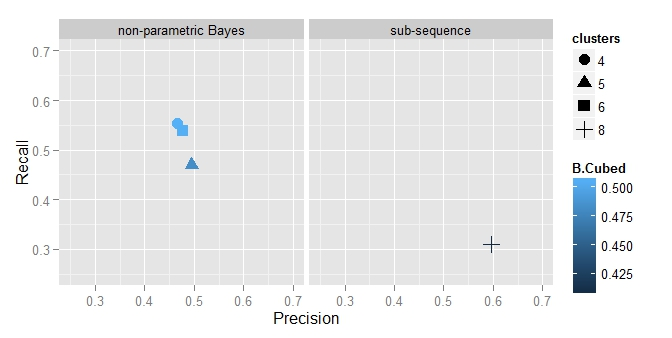
\includegraphics[width=\columnwidth]{fig/hepC.jpeg}}
\caption{Comparison of semiparametric clustering with a reported benchmark}
\label{hepC}
\end{center}
\vskip -0.2in
\end{figure}

\begin{table}[ht]
\caption{Validation scores for spectral (SC) and nonparametric Bayes (Bayes) clustering on all hepatitis patients.}
\label{scBayestable}
\vskip 0.15in
\begin{center}
\begin{small}
\begin{sc}
\begin{tabular}{lcccr}
\hline
\abovespace\belowspace
method	& k	& P	& R	& B-Cubed \\
\hline
\abovespace
sub-sequence	& 8& 0.60& 0.31& 0.41 \\
SP-B(PLT)		& 5& 0.49& 0.42& 0.45 \\
\textbf{SP-B}	        & \textbf{4}& \textbf{0.47}& \textbf{0.55}& \textbf{0.51 }\\
SP-B	        & 5& 0.50& 0.47& 0.48 \\

\belowspace
\textbf{SP-B}	        &\textbf{ 6}& \textbf{0.48}& \textbf{0.54}& \textbf{0.51} \\
\hline
\end{tabular}
\end{sc}
\end{small}
\end{center}
\vskip -0.1in
\end{table}

Also, we apply our method to the entire data set, including those on interferon therapy and patients with hepatitis B, and compare it with an alternative nonparametric method, spectral clustering.  The results appear in Figure~\ref{allHep} and are detailed in Table~\ref{allHepTable}.

\begin{figure}[t]
\vskip 0.2in
\begin{center}
\centerline{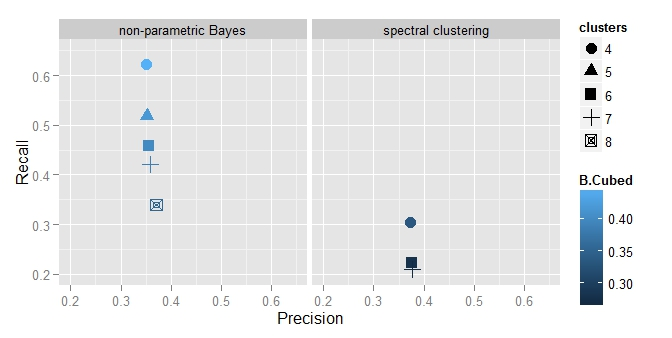
\includegraphics[width=\columnwidth]{fig/allHep.jpeg}}
\caption{B-cubed value for different methods and $k$ values for the hepatitis data set}
\label{allHep}
\end{center}
\vskip -0.2in
\end{figure}


\begin{table}[ht]
\caption{B-cubed value for spectral (SP-SC) and nonparametric Bayes (SP-B) clustering, all hepatitis patients.}
\label{allHepTable}
\vskip 0.15in
\begin{center}
\begin{small}
\begin{sc}
\begin{tabular}{lcccr}
\hline
\abovespace\belowspace
method	& k	& P	& R	& B-Cubed \\
\hline
\abovespace
SP-SC	         & 6	& 0.38& 0.22& 0.28\\
SP-SC	         & 7	& 0.38& 0.21& 0.27\\
\textbf{SP-B }       & \textbf{4}	& \textbf{0.35}& \textbf{0.62}& \textbf{0.45}\\
SP-B	     & 5	& 0.35& 0.52& 0.42\\
SP-B	     & 6	& 0.36& 0.46& 0.40\\
\belowspace
SP-B	     & 7	& 0.36& 0.42& 0.39\\
\hline
\end{tabular}
\end{sc}
\end{small}
\end{center}
\vskip -0.1in
\end{table}


\subsection{Diabetes Experiments}
The glucose testing data was processed before state estimation.  Creating a new vector, we set the observation value to the number of days contiguous tests were ordered.  For example, and measurement sequence of $[1,0,0,0,1,1,1,1]$ would consist of two observations, 1 and 4.  We estimated $n$, the number of states for the models using a non-parametric Bayesian density estimator.  Since the number of states and the continuous nature of the model should not be too large, the upper-bound on the number for density estimation was set to a maximum of five.


\subsubsection{Intrinsic Validation}
When a gold standard is unavailable to evaluate clustering performance, heuristics can be used to assess the intrinsic quality of clusters.  For each point in the data set, the silhouette method is defined by the different of average dissimilarity of a point to members or its own cluster with that of the `neighboring' cluster over the max of these two dissimilarity measures.

Based on the results of applying our clustering approach to the glucose testing data, Figure~\ref{sil} shows the silhouette for the assignments and Table~\ref{stats} shows cluster averages including: number of members, total glucose tests, number of hospital admissions, entropy of the measurement sequence, and fraction of days measured.

\begin{figure}[t]
\begin{center}
\centerline{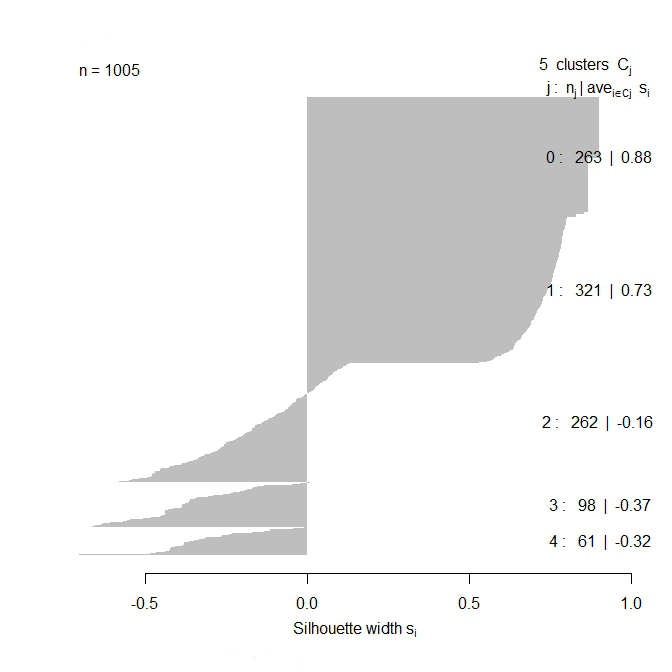
\includegraphics[width=\columnwidth]{fig/sil.jpeg}}
\caption{Silhouettes by cluster for 4-state model.}
\label{sil}
\end{center}
\vskip -0.2in
\end{figure}


\begin{table}[ht]
\caption{Time series statistics aggregated by cluster}
\label{stats}
\vskip 0.15in
\begin{center}
\begin{small}
\begin{sc}
\begin{tabular}{lccccr}
\hline
\abovespace\belowspace
k 	&n 	&Tests 	&Stays 	&Entropy 	&Fraction \\
\hline
\abovespace
0	&263	&8.6	&7.81	&0.05	&0.01\\
1	&321	&39.64	&16.98	&0.14	&0.04\\
2	&262	&22.00	     &13.53	&0.10	&0.02\\
3	&98	    &24.77	&11.38	&0.10	&0.02\\
4	&61	    &16.74	&7.69	&0.08	&0.02\\
\belowspace
T 	&1005	&24.08	&12.57	&0.10	&0.02\\
\hline
\end{tabular}
\end{sc}
\end{small}
\end{center}
\vskip -0.1in
\end{table}





\section{Clinical Relevance}
\label{clin}
%\begin{figure}[ht]
%\vskip 0.2in
%\begin{center}
%\centerline{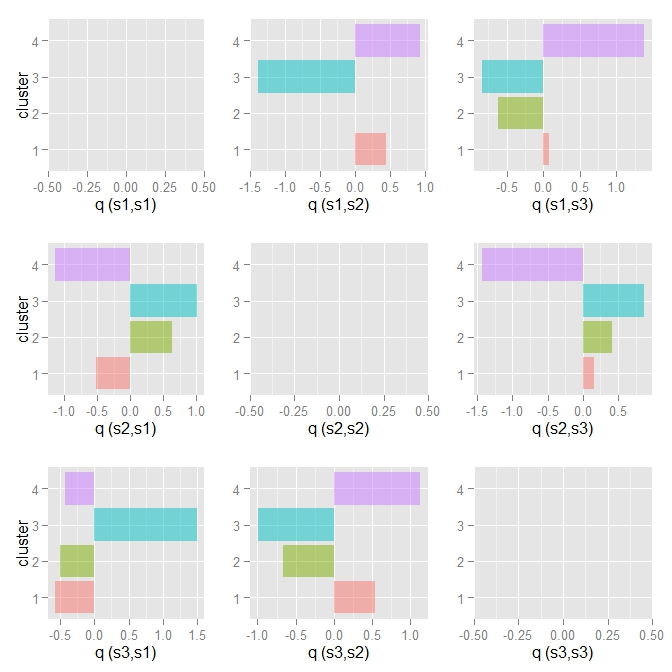
\includegraphics[width=\columnwidth]{fig/qmatrix.jpeg}}
%\caption{Historical locations and number of accepted papers for International
%  accepted papers for ICML 2008 was unknown and instead estimated.}
%\label{icml-historical}
%\end{center}
%\vskip -0.2in
%\end{figure}
 Using biopsy results as a gold standard for clustering, our results indicate over a 20\% relative improvement on a benchmark (.41-.51 b-cubed) for detecting liver fibrosis in a subset of hepatitis C patients from the liver disease data.  Relative to the results based on the whole data set, better performance is achieved for the hepatitis C patients without interferon therapy.  This is not surprising.  Interferon therapy is physiologically disruptive and the reason for the selection criteria in the benchmark set.  However, despite the introduction of this noise, our method performs better on the group of all patients than the benchmark performs on only this subset of more predictable patients.

Of clinical relevance was an `extreme' effect that could be viewed among different clustering runs.  The lowest risk cluster, designated by the highest proportion of patients with no or minor fibrosis, reported 80-94\% purity and was composed of 15-25 percent of the patients for a $4<k<6$.  This cluster represents patients with very low risk of fibrosis, and may be good candidates for delaying biopsy.

Additionally, for an inpatient population, we can detect recognizable differences in the incidence of physicians' orders for glucose tests among discovered groups that can be visualized. We also assess the performance of pairing temporal abstraction with a non-parametric Bayesian clustering.  It conveniently eliminates the need to estimate $k$, and  performed better that spectral clustering on the hepatitis data set.

The glucose test experiment demonstrates two distinct groups with average silhouette value of .73 and .88 and accounting for almost 60\% of the population sampled.  These two groups show the most dramatic differences in average sequence entropy (0.05-0.14), the fraction of days measured (0.01-0.04) and the number of tests (8.60-39.64).  When the original sequence is viewed as a heat map, a typical patient's sequence in the low risk group will consists of sparse signals, with only the initial visit consisting of more that one contiguous tests.  However, patients in group have testing patterns that are longer in duration, showing streaks of contiguous testing, and suggesting they are more prone to diabetes related morbidity.  Patients in the remaining clusters represent an intermediate between these two groups and mixtures of testing patterns.

Since diabetes is undiagnosed in millions of Americans, and preventative treatment can help avoid serious effects and avoidable costs to providers, using administrative data, such as glucose testing pattern, may prove useful for disease surveillance.  For example, an insurance provider does not have access to lab results, but they will have a signal for per patient tests, information on demographic risk factors, and other billing diagnoses for patients. The ability to leverage high level signals with demographic and other claims data to flag prediabetes or undiagnosed diabetes could be useful for developing cost-savings strategies that improve health outcomes in parallel.


\section{Conclusions and Future Work}
\label{conc}
We describe a new method to model patient disease dynamics with several key features.  First, we apply continuous-time Markovian models for modeling disease dynamics, which avoids some of the limitations of discrete-time approaches when a dynamic process evolves at different time granulations, and when observations are irregularly sampled and missing not at random.  Second, non-parametric Bayesian clustering methods avoid the problem of identifying the number of clusters a priori, inferring the appropriate number of mixture component as a function of the sample size.

 The limitations of this work are mainly attributed to the temporal modeling steps. Continuous-time models bring us closer to a natural representation, but they are still inconsistent with the real-world. For example, the in the model the instantaneous probability for a state transition is the same for the entire duration of occupation.  Another issue is that not all patient models converged during the abstraction step.  Although this impacted only small fraction of the total patients, it is a key limitation to the method. 

  Immediate next steps are to extend temporal abstraction to continuous-time HMMs.  Also, we feel that external validation metrics for cluster assessment are fundamentally weak for many problems where clusters are not categorical, and rather a graded interval. In terms of intrinsic evaluation, heuristics such as the silhouettes are also limited.  Instead of developing one more metric, we propose a visualization tool to enable the browsing of temporal clustering results and feel this would be more useful for system development and is another direction for our future work.



\bibliography{example_paper}
\bibliographystyle{icml2013}

\end{document}

